%%%%%%%%%%%%%%%%%%%%%%%%%%%%%%%%%%%%%%%%%%%%%%%%%%%%%%%%%%%%%%%%%%%%%%%%%%% 
% 
% Generic template for TFC/TFM/TFG/Tesis
% 
% By:
% + Javier Macías-Guarasa. 
% Departamento de Electrónica
% Universidad de Alcalá
% + Roberto Barra-Chicote. 
% Departamento de Ingeniería Electrónica
% Universidad Politécnica de Madrid   
% 
% Based on original sources by Roberto Barra, Manuel Ocaña, Jesús Nuevo,
% Pedro Revenga, Fernando Herránz and Noelia Hernández. Thanks a lot to
% all of them, and to the many anonymous contributors found (thanks to
% google) that provided help in setting all this up.
% 
% See also the additionalContributors.txt file to check the name of
% additional contributors to this work.
% 
% If you think you can add pieces of relevant/useful examples,
% improvements, please contact us at (macias@depeca.uah.es)
% 
% You can freely use this template and please contribute with
% comments or suggestions!!!
% 
%%%%%%%%%%%%%%%%%%%%%%%%%%%%%%%%%%%%%%%%%%%%%%%%%%%%%%%%%%%%%%%%%%%%%%%%%%% 

\chapter{Improving Multi-Agent Motion Prediction with Heuristic Proposals and Motion Refinement}
\label{cha:improving_multi_agent}

\begin{FraseCelebre}
	\begin{Frase}
		Solo sé que no sé nada.
	\end{Frase}
	\begin{Fuente}
		Sócrates a Platón \\
		Diálogos de Platón
	\end{Fuente}
\end{FraseCelebre}

\section{Introduction}
\label{sec:7_introduction}

This is the last and most advanced \ac{MP} algorithm proposed in this thesis. Based on our previously stated map baseline, we aim to get an efficient model that consider more information about the agents, HD map topological and semantic information (in addition to the previously stated geometric features) and contextual interactions. Note that obtaining and fusing this information (\eg \ actor-to-actor, map-to-actor) is a research topic by itself \cite{varadarajan2022multipath++, zeng2021lanercnn, liang2020learning} and a core part in the \ac{ADS} pipeline. Here we identify a bottleneck for efficient real-time applications \cite{KATRAKAZAS2015416realtime, gomez2021smartmot}, as usually, more (complex) data-inputs implies higher model complexity and inference time \cite{gao2020vectornet}. 

Predicting the future trajectories of the agents without considering their nature might not be optimal (\eg \ predicting on a pedestrian, a cyclist or a vehicle using the same logic). For this reason, we integrate additional features related to the type and properties of agents (also referred as metadata in the literature). Moreover, we also compute heuristic scene understanding to constrain the model predictions towards the real scene geometry (\eg \ plausible centerlines and lanes), including lane and boundary topological information or presence of an intersection. 
As stated by \cite{zhang2022banet}, only using lane centerline as input to get the embedding feature of vector map nodes is not enough. The lane centerline can only provide the
topology of the lanes, and other elements of the vector map also contain rich information. For example, the lane boundary can provide traffic rule constraint information such as whether it is possible to conduct the lane change behaviour or not (dashed vs solid line, yellow vs white, etc.). When considering such amount of information, specifically in terms of physical context and interactions, most \ac{SOTA} methods require an overwhelming model complexity which can be inefficient in terms of computation \cite{gao2020vectornet, walters2020trajectory, can2022maps}.

\section{Our proposal}
\label{sec:7_our_proposal}

To address the aforementioned \ac{SOTA} limitations, we propose a model \cite{gomez2023improving} to achieve accurate motion prediction, yet, using light-weight transformer-based models for social encoding, \acp{GNN} for context interaction, enhanced heuristic proposals and motion refinement, reducing notably the complexity of our model with respect to previous methods such as GANet \cite{wang2022ganet} to avoid these possible constraints. Figure \ref{fig:chapter_7_Improving_Multi_Agent/CVPR_2023} illustrates the overall pipeline. We make the following contributions:

\begin{enumerate}
	\item We present a \ac{SOTA} method on the Argoverse 2 Motion Forecasting Benchmark, one of the most recent and challenging vehicle \ac{MP} datasets.
	\item Our model uses various attention mechanisms with GNNs, and a motion refinement module to further improve temporal consistency.
	\item In comparison to previous methods that rely only on past trajectories and HD map, we additionally use information about the agents (\eg \ type of agent) and the scene geometry (\eg \ lane distribution and possible goal points).
	\item Our method reduces in millions of parameters previous methods such as GANet \cite{wang2022ganet}, and improves over LaneGCN \cite{liang2020learning}.
	\item Finally, we provide an open-source framework for MP.
\end{enumerate}

Throughout this Chapter we will explain the different modules of the proposed \ac{MP} method, which are: 1) \textbf{Social Encoder}, which uses the agent past trajectories (relative displacements and additional metadata such as the type (\eg \ car, cyclist, pedestrian) and category, from less to more important) and the corresponding heuristic lane proposals to compute the social features, 2) \textbf{Map Encoder}, that constructs a lane graph from the HD Map and uses a LaneConv operator \cite{liang2020learning} to extract lane node features, 3) \textbf{Fusion Cycle}, responsible for fusing agents and map latent features, 4) \textbf{Goal Areas estimation}, to predict some goals and their surrounding  (area) features are aggregated to the agents, 5) \textbf{Multimodal Decoder}, which uses the latent actors with deep area context to generate reliable multi-modal predictions and 6) \textbf{Motion Refinement}, in charge of enhancing the quality of the future trajectories taking into account the past trajectories, actors latent features and preliminary predicted trajectories.

\begin{figure}[h] 
	\centering
	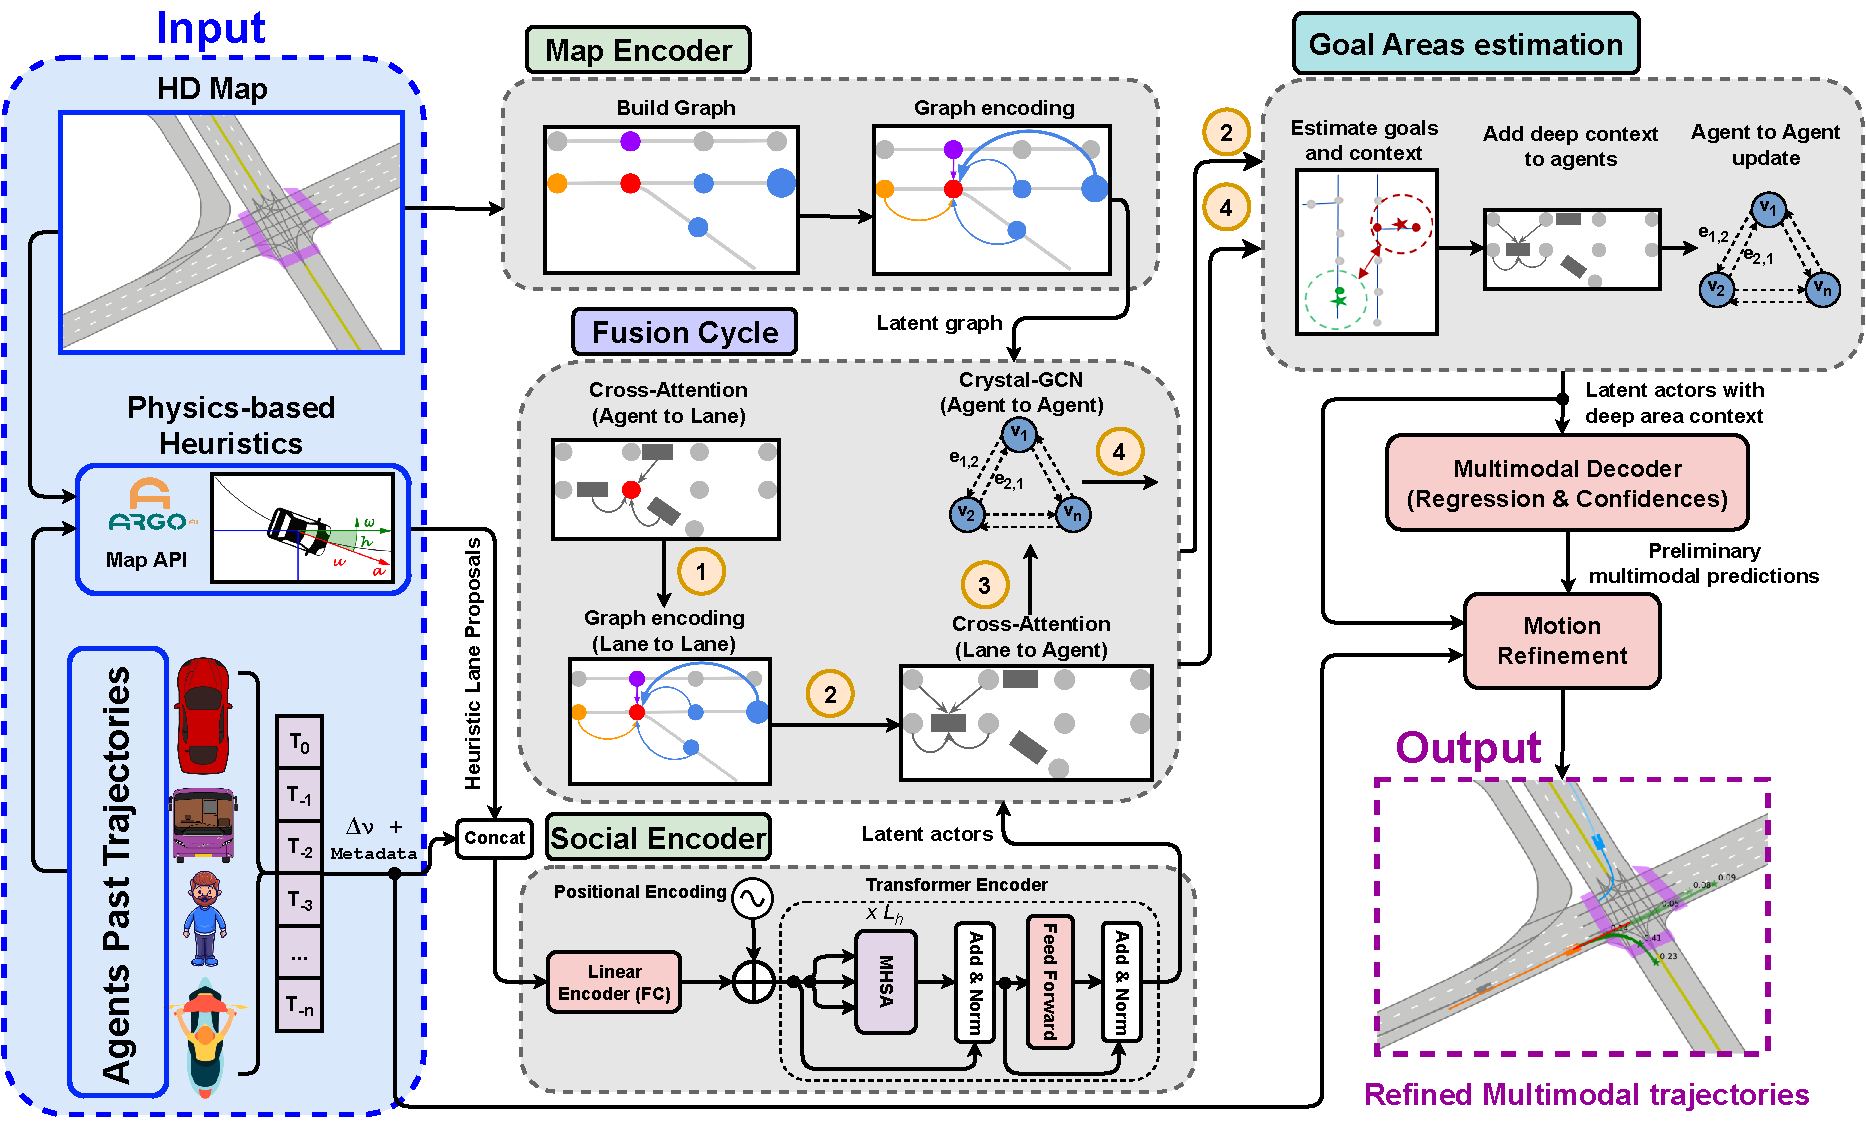
\includegraphics[width=\textwidth]{chapter_7_Improving_Multi_Agent/CVPR_2023.pdf}
	\caption{Overview of our Motion Prediction model including Fusion Cycle, Heuristic Proposals and Motion Refinement}
	\label{fig:chapter_7_Improving_Multi_Agent/CVPR_2023}
\end{figure}

\subsection{Preprocessing of past trajectories and heuristic proposals}
\label{subsec:7_improving_efficiency_preprocessing}

The social preprocessing step proposed in this model is slightly different to our previous methods where we only considered those agents that have information over the full history horizon. Now, given the complexity of Argoverse 2, an agent that recently appeared in the scene, even if it was not observed over the whole full sequence spectrum, or even it was occluded for a few timestamps, it can be really relevant to determine the future behaviour of another agent. To this end, as proposed by multiple methods \cite{liang2020learning, schmidt2022crat}, we consider all agents that are observable at \textit{t=0}, handling those agents that are not observed over the full sequence spectrum (observation length = \textit{$obs_{len}$} + prediction length = \textit{$pred_{len}$}) by concatenating a binary flag $b_i^t$ that indicates if the agent is padded or not. On top of that, we only consider the dynamic agents of the scene (vehicles, pedestrians, motorcyclists, cyclists and buses) and discard unknown or static objects (background, construction or riderless bicycle), since dynamic (which can be stopped or not) are the most relevant for the \ac{MP} task. Given these final agents, we follow the same principles of translation and rotation invariant, as well as relative displacements, to compute the input past trajectories. On top of that, we additionally compute and codify the object type (bus, pedestrian, vehicle, cyclist) and agent importance (unscored, scored and focal track) as additional metadata. As described by Argoverse 2, each track is assigned one of the following labels, which dictate scoring behavior in the Argoverse 2 challenges:

\begin{enumerate}
	\item Track fragment: Lower quality track that may only contain a few timestamps of observations.
	\item Unscored track: Unscored track used for contextual input.
	\item Scored track: High-quality tracks relevant to the agent.
	\item Focal track: The primary track of interest in a given scenario - scored in the single-agent prediction challenge.
\end{enumerate}

We can appreciate how, in addition to the attention mechanisms of the model which are responsible of computing the most relevant features, the aforementioned track category serves as a good guidance as preliminary information to refer the importance of a specific agent with respect to another one.

In terms of physical information, we aim to increase the number of features of the HD Map as well as its corresponding interactions with the social features. Then, we focus on \textbf{Graph-based} methods \cite{zeng2021lanercnn} which construct graph-structured representations from the HD maps, which preserve the connectivity of lanes, and therefore the geometry of the scene. VectorNet \cite{gao2020vectornet} is one of the first works in this direction, where the authors propose to encode map elements and actor trajectories as polylines and then use a global interactive graph to fuse map and actor features. We find especially related LaneGCN \cite{liang2020learning}, a method that constructs a map node graph and proposes a novel graph convolution. In that sense, we follow the same principles than these well-established baselines by adopting simple form of vectorized map data as our representation of HD maps. In this case, the map data is represented as a set of polylines (lanes) and
their connectivity, where each lane contains a centerline (sequence of 2D \ac{BEV} points), arranged following the lane direction. For any two lanes which are directly reachable, 4 types of connections are given: predecessor, successor, left neighbour and right neighbour.

Moreover, we propose the use of preliminary plausible area information in a similar way to the heuristic proposals illustrated in Section \ref{subsubsec:6_efficient_baselines_preprocessing_map}. We follow the same heuristic (filter the agent, calculate the future travelled distance by means a CA model, get all candidates within a bubble, given the agent last observation and Manhattan distance, etc) to compute the most plausible future centerlines for the corresponding agent. It must be considered that in Argoverse 2 the number of categories is modified to 5 (vehicles, pedestrians, motorcyclists, cyclists and buses) insteaf of only 1 (vehicle) in the case of most vehicle \ac{MP} datasets, including Argoverse 1. So, no centerlines proposals are considered (then, they are created virtually and padded as stated in previous sections) since we assume that pedestrians are not walking on the road, but on the pedestrian crossings or sidewalks. In future works we will work on integrating specific physical information depending on the object type as preliminary map features. Nevertheless, in this particular case, thanks to a more realistic representation of the HD map, we include additional metadata such as lane type (bus, bike, vehicle), presence of intersection (binary flag) or boundaries mark type (dash, solid, yellow), along with the aforementioned centerline relative displacements. 

\subsection{Social Encoder}
\label{subsubsec:7_improving_efficiency_social_encoder}

In terms of social encoding, in order to capture more complex features for subsequent features fusion and interaction, we initially adopted GANet \cite{wang2022ganet}, based on LaneGCN \cite{liang2020learning}, to encode motion history and scene context for its outstanding performance. In this backbone (given the aforementioned social input: translation and rotation invariant with respect to a target agent, and relative displacements), LaneGCN makes use of use a network with $3$ groups/scales of 1D convolutions 1D CNN to process the trajectory input for its effectiveness in extracting multi-scale features and efficiency in parallel computing. The output is a well-structured feature map, whose element at $t=0$ is used as the actor feature. The network has $3$ groups/scales of 1D convolutions. Then, a Feature Pyramid Network (FPN) \cite{lin2017feature} to fuse the multi-scale features, and apply another residual block to obtain the output tensor. Moreover, GANet applies an \ac{LSTM} network on FPN output features and use two identical parallel networks to enhance the motion history encoding.

Regarding this, we aimed to improve social encoding taking into account that in spite the fact that \acp{LSTM} became popular because they could solve the problem of vanishing gradients, they suffer from \textit{short-term memory} due to the vanishing gradient problem, as well as require a lot of resources to get trained and become ready for real-world applications. In particular, they need high memory-bandwidth because of linear layers present in each cell which the system usually fails to provide for. To solve that, we replace the motion encoder proposed by \cite{wang2022ganet} for a transformer encoder, which is faster than \ac{RNN}-based models as all the input is ingested once, decreasing the computational complexity. On the other hand, even though the preliminary lane proposals represent physical information, they are quite related to the future intentions of the social information. Then, as depicted in Figure \ref{fig:chapter_7_Improving_Multi_Agent/CVPR_2023}, we concatenate the agents past trajectories, additional social metadata and heuristic map proposals (including semantic and topological metadata), which is processed by a linear embedding. Then, positional encoding is added to the output embedding explicitly to retain the information regarding the order of past trajectories and future preliminar steps. Finally, these latent features feed the transformer encoder, leveraging the self-attention mechanism and positional encoding to learn complex and dynamic patterns from long-term time series data. 

\subsection{Map preprocessing and encoding}
\label{subsec:7_improving_efficiency_map_preprocessing_and_encoding}

In terms of physical context, we adopt MapNet \cite{liang2020learning} backbone to encode the scene context for its outstanding performance. %It learns good lane representations which are computationally efficient and preserve map topology. We use a multi-scale LaneConv network to encode the vectorized map data, which is consisted of lane centerlines and their connectivity. We construct a lane node graph from the map data. A lane node is a short lane segment between two consecutive points of the lane centerline, which is represented by the location (the averaged coordinates of its two endpoints) and the shape (the vector between its two endpoints). 
While other approaches encode the map as a raster image and apply 2D convolutions to extract features, MapNet consists of two steps:

\begin{itemize}
	\item Build a lane graph from vectorized map data
	\item Apply a LaneConv operator to the lane graph to output the map features
\end{itemize}

\begin{figure}[h] 
	\centering
	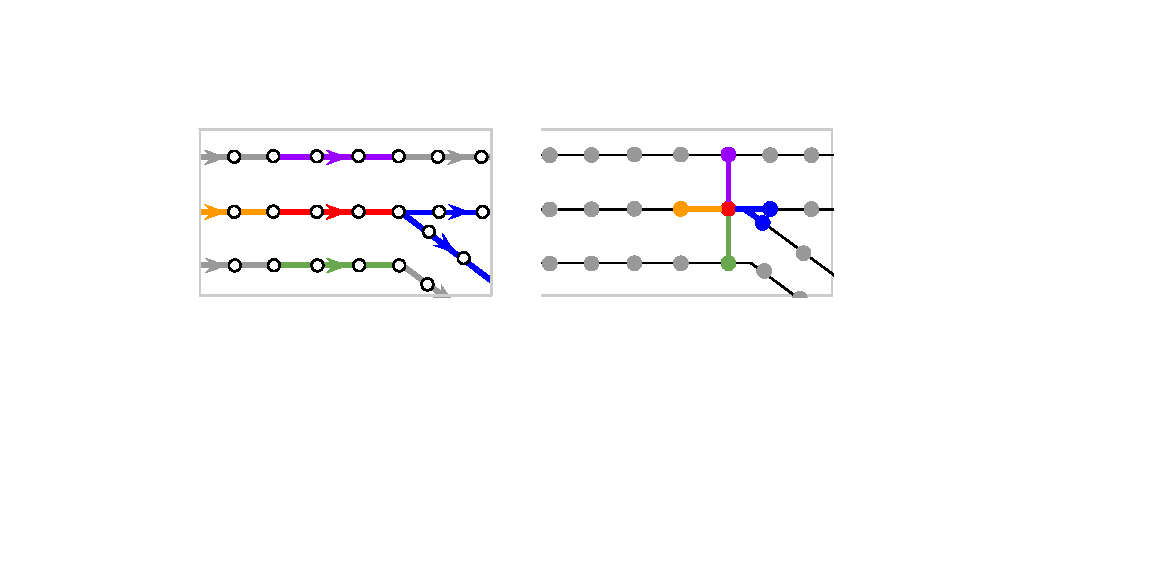
\includegraphics[width=0.8\textwidth]{chapter_7_Improving_Multi_Agent/lanegcn_map_representation.pdf}
	\caption{Lane graph construction from vectorized map data}
	Source: \textit{Learning lane graph representations for motion forecasting} \cite{liang2020learning}
	\label{fig:chapter_7_Improving_Multi_Agent/improving_efficiency_lanegcn_map_representation}
\end{figure}

As observed in Figure \ref{fig:chapter_7_Improving_Multi_Agent/improving_efficiency_lanegcn_map_representation}, the map data is represented as a set of lanes and their connectivity. Each lane contains a centerline, \ie \ a sequence of 2D BEV points, which are arranged following the lane direction. For any two lanes which are directly reachable, $4$ types of connections are given: \textit{predecessor}, \textit{successor}, \textit{left neighbour} and \textit{right neighbour}. Given a lane $A$, its predecessor and successor are the lanes which can directly travel to $A$ and from $A$ respectively. Left and right neighbours refer to the  lanes which can be directly reached without violating traffic rules. This simple map format provides essential geometric and semantic information for \ac{MP}, as vehicles generally plan their routes by reference to lane centerlines and their connectivity. 

In order to conduct the Lane Graph construction, we first define a lane node as the straight line segment formed by any two consecutive points (grey circles in Figure \ref{fig:chapter_7_Improving_Multi_Agent/improving_efficiency_lanegcn_map_representation}) of the centerline. The location of a lane node is the averaged coordinates of its two end points. Following the  connections between lane centerlines, we also derive $4$ connectivity types for the lane nodes, \ie \ \textit{predecessor}, \textit{successor}, \textit{left neighbour} and \textit{right neighbour}. For any lane node $A$, its predecessor and successor are defined as the neighbouring lane nodes that can travel to $A$ or from $A$ respectively. Note that one can reach the first lane node of a lane $l_{A}$ from the last lane node of lane $l_{B}$ if $l_{B}$ is the predecessor of $l_{A}$. Left and right neighbours are defined as the spatially closest lane node measured by $\ell_2$ distance on the left and on the right neighbouring lane respectively. We denote the lane nodes with $V \in \mathbb{R}^{N \times 2}$, where $N$ is the number of lane nodes and the $i$-th row of $V$ is the BEV coordinates of the $i$-th node. We represent the connectivity with $4$ adjacency matrices $\{A_i\}_{ i \in \{\text{pre}, \text{suc}, \text{left}, \text{right}\} }$, with $A_i \in \mathbb{R}^{N \times N}$. We denote $A_{i, jk}$, as the element in the $j$-th row and $k$-th column of $A_i$. Then  $A_{i, jk} = 1$ if node $k$ is an $i$-type neighbor of node $j$. 

\subsubsection{LaneConv Operator}
\label{subsubsec:7_improving_efficiency_lane_conv}

A natural operator to handle lane graphs is the graph convolution \cite{shuman2013emerging}.
The most widely used graph convolution operator \cite{kipf2016semi} is defined as $Y = LXW$, where $X \in \mathbb{R}^{N \times F}$ is the node feature, $W \in \mathbb{R}^{F \times O}$ is the weight matrix, and $Y \in \mathbb{R}^{N \times O}$ is the output. The graph Laplacian matrix $L \in \mathbb{R}^{N \times N}$ takes the form $L = D^{-1/2}(I + A)D^{-1/2}$, where $I$, $A$ and $D$ are the identity, adjacency and degree matrices respectively. $I$ and $A$ account for self connection and connections between different nodes. All connections share the same weight $W$, and the degree matrix $D$ is used to normalize the output. However, this vanilla graph convolution is inefficient in our case due to the following reasons. First, it is not clear what kind of node feature will preserve the information in the lane graphs. Second, a single graph Laplacian can not capture the connection type, \ie \ losing the directional information carried by the connection type. Third, it is not straightforward to handle long range dependencies within this form of graph convolution. Motivated by these challenges, we introduce our novel specially designed operator for lane graphs, called \textit{LaneConv}.

\paragraph{Node Feature}
\label{par:7_improving_efficiency_node_feature}

We first define the input feature of the lane nodes. Each lane node corresponds to a straight line segment of a centerline. To encode  all the lane node information, we need to take into account both the shape (size and orientation) and the location (the coordinates of the center) of the corresponding line segment. We parameterize the node feature as follows:

\begin{equation}
	\mathbf{x}_i = \text{MLP}_\text{shape} \left( \mathbf{v}_i^{\text{end}} - \mathbf{v}_i^{\text{start}} \right)
	+ \text{MLP}_{\text{loc}}\left(\textbf{v}_i\right)
	\label{eqn:node_feat}
\end{equation}

where $\text{MLP}$ indicates a multi-layer perceptron and the two subscripts refer to shape and location, respectively.  $\textbf{v}_i$ is the location of the $i$-th lane node, \ie, the center between two end points, $\mathbf{v}_i^{\text{start}}$ and $\mathbf{v}_i^{\text{end}}$ are the BEV coordinates of the node $i$'s starting and ending points, and $\mathbf{x}_i$ is the $i$-th row of the node feature matrix $X$, denoting the input feature of the $i$-th lane node.

\paragraph{LaneConv}
\label{par:7_improving_efficiency_lane_conv}

The node feature above only captures the local information of a line segment.
To aggregate the topology information of the lane graph at a larger scale,
we design the following LaneConv operator:

\begin{equation}
	Y = X W_0 + \sum_{i \in \{ \text{pre}, \text{suc}, \text{left}, \text{right} \}} {A_{i} X W_{i}}
	\label{eqn:laneconv}
\end{equation}

where $A_{i}$ and $W_i$ are the adjacency  and the weight matrices corresponding to the $i$-th connection type respectively. Since we order the lane nodes from the start to the end of the lane, $A_{\text{suc}}$ and $A_{\text{pre}}$ are matrices obtained by shifting the identity matrix one step towards upper right (non-zero superdiagonal) and lower left (non-zero subdiagonal). $A_{\text{suc}}$ and $A_{\text{pre}}$ can propagate information from the forward and backward neighbours whereas $A_{\text{left}}$ and $A_{\text{right}}$ allow information to flow from the cross-lane neighbours. It is not hard to see that our LaneConv builds on top of the general graph convolution and encodes more geometric (\eg \ connection type/direction) information.

\paragraph{Dilated LaneConv}
\label{par:7_improving_efficiency_dilated_laneconv}

Since motion forecasting models usually predict the future trajectories of actors with a time horizon of several seconds, actors with high speed could have moved a long distance.
Therefore, the model needs to capture the long range dependency along the lane direction for accurate prediction. In regular grid graphs, a dilated convolution operator \cite{yu2015multi} can effectively capture the long range dependency by enlarging the receptive field. Inspired by this operator, we propose the \textit{dilated LaneConv} operator to achieve a similar goal for irregular graphs. 

In particular, the $k$-dilation LaneConv operator is defined as follows:

\begin{equation}
	Y = XW_0 + A_{\text{pre}}^k X W_{\text{pre},k} + A_{\text{suc}}^k X W_{\text{suc},k}
	\label{eqn:dilated_laneconv}
\end{equation}

where $A_{\text{pre}}^k$ is the $k$-th matrix power of $A_{\text{pre}}$. 
This  allows us to directly propagate information along the lane for $k$ steps, with $k$ a hyperparameter. Since $A_{\text{pre}}^k$ is highly sparse, one can efficiently compute it using sparse matrix multiplication. Note that the dilated LaneConv is only used for predecessor and successor, as the long range dependency is mostly along the lane direction.

\subsubsection{LaneGCN}
\label{subsubsec:4_improving_efficiency_lanegcn}

\begin{figure}[t]                               
	\begin{center}
		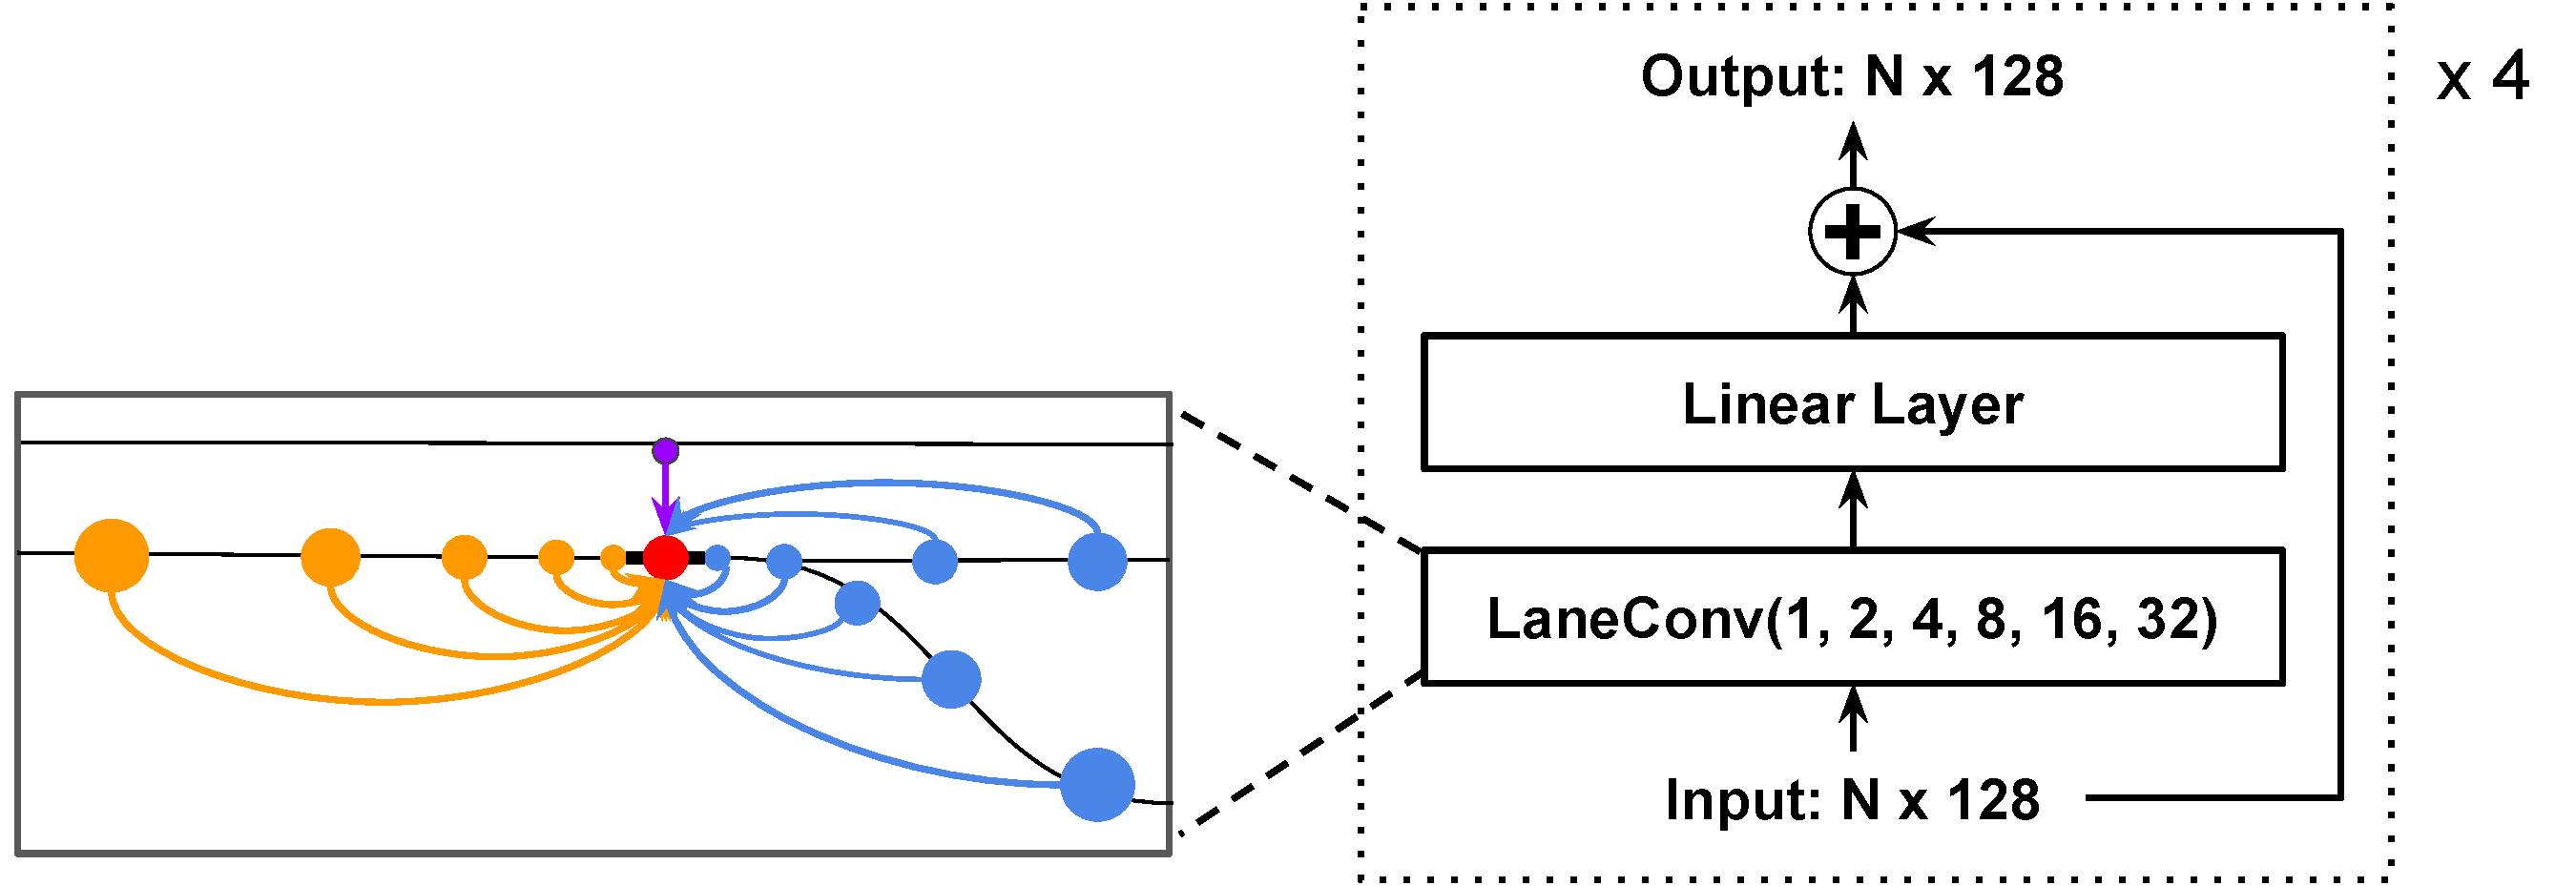
\includegraphics[width=0.8\linewidth]{chapter_7_Improving_Multi_Agent/lanegcn_scheme.pdf}
	\end{center}
	\caption[LaneGCN architecture]{LaneGCN architecture. LaneGCN is a stack of 4 multi-scale LaneConv residual blocks, each of which consists of a LaneConv(1,2,4,8,16,32) and a linear layer with a residual connection.}
	Source: \textit{Learning lane graph representations for motion forecasting} \cite{liang2020learning}
	\label{fig:chapter_7_Improving_Multi_Agent/improving_efficiency_lanegcn}
\end{figure}

Based on the dilated LaneConv, we further propose a multi-scale LaneConv operator and use it to build our LaneGCN.
Combining Eq. (\ref{eqn:laneconv}) and (\ref{eqn:dilated_laneconv}) with multiple dilations, we get a multi-scale LaneConv operator with $C$ dilation sizes as follows:

\begin{equation}\label{eqn:dilated_laneconv_final}
	Y = XW_0 + \sum_{i \in \{ \text{left}, \text{right} \}} {A_{i} X W_{i}}
	+ \sum_{c=1}^{C} {\left( A_{\text{pre}}^{k_{c}} X W_{\text{pre},k_{c}} + A_{\text{suc}}^{k_{c}} X W_{\text{suc},k_{c}} \right)},
\end{equation}
where $k_c$ is the $c$-th dilation size. We denote  $\text{LaneConv}(k_1, \cdots, k_C)$ this multi-scale layer. 

\subsection{Enhanced Actor-Map Fusion Cycle}
\label{subsubsec:4_improving_efficiency_enhanced_fusion_cycle}

Once both the map and social latent features are computed, we obtain a 2D feature matrix $X$ where each row $X_i$ indicates the feature of the $i$-th actor, and a 2D matrix $Y$ where each row $Y_i$ indicates the feature of the $i$-th lane node. Then, we make use of the well-established actor-map fusion cycle \cite{liang2020learning} (also referred as FusionNet in the literature) that transfers and aggregates feature among actors and lane nodes. The behaviour of an actor strongly depends on its context, \ie, other actors and the map. Although the interactions between actors has been explored by previous work, the interactions between the actors and the map, and map conditioned interactions between actors have received much less attention. FusionNet makes use of spatial attention and LaneGCN to capture a complete set of actor-map interactions, as observed in Figure \ref{fig:chapter_7_Improving_Multi_Agent/CVPR_2023}.

FusionNet makes use of a stack of four fusion modules to capture all information flows between actors and lane nodes, \ie, (1) Actors to Lanes (A2L), (2) Lanes to Lanes (L2L), (3) Lanes to Actors (L2A) and (4) Actors to Actors (A2A). This order is not coincidence. Assuming several agents are on the road and all of them have a web service that provides detailed information about geographical regions and sites worldwide (\eg \ Google Maps):

\begin{itemize}
	\item First, agents introduce their real-time traffic information to lane nodes, such as blockage, presence of an accident, etc. In other words, the HD map information is updated with the traffic information of the agents.
	\item The HD map information of a particular node is propagated to the immediate neighbours, in such a way ...
	\item ... further agents are updated with the information of surrounding map nodes, which were previously updated by neighboring nodes.
	\item Finally, A2A concludes the actor-map fusion cycle handling the interactions between actors and produces the output actor features.
	
\end{itemize}

We implement L2L using another LaneGCN, which has the same architecture as the one used in our MapNet. Regarding the A2L, L2A and A2A modules, \cite{liang2020learning} applies a spatial attention layer as defined in Section \ref{subsec:3_attention}. Taking the first module (A2L) as en example, given an actor node $i$, we aggregate the features from its context lane nodes $j$ as follows:

\begin{equation}
	\mathbf{y}_i = \mathbf{x}_i W_0 + \sum_j \phi ( \text{concat} (\mathbf{x}_i, \Delta_{i,j}, \mathbf{x}_j) W_1) W_2
	\label{equ:attention}
\end{equation}

where $\mathbf{x}_i$ represents the feature of the $i$-th node, $W$ a weight matrix, $\phi$ the composition of layer normalization and ReLU, and $\Delta_{ij} = \text{MLP}(\mathbf{v}_j - \mathbf{v}_i)$, where $\mathbf{v}$ denotes the node location.

The context nodes are defined to be the lane nodes whose $\ell_2$ distance from the actor node $i$ is smaller than a threshold. Each of A2L, L2A and A2A has two residual blocks, which consist of a stack of the proposed attention layer and a linear layer, as well as a residual connection. 

Nevertheless, as observed in our model (Figure \ref{fig:chapter_7_Improving_Multi_Agent/CVPR_2023}), once implemented FusionNet to compute actor-map interactions, we substitute the final module that models Actor to Actor interactions with a Graph Convolution Operator (GCN), inspired in our previous proposed efficient baselines (Figure \ref{fig:chapter_6_Efficient_Baselines/TITS_2023}). %Further results (Section \ref{sec:5_motion_prediction_datasets}) will illustrate that replacing the final spatial attention among agents by an efficient graph operator preserves global agent interaction while enhances the whole model in terms of computational complexity and inference time.

\begin{comment}
	\subsection{Decoding Module}
	
	\subsubsection{Goals Prediction and Filtering}
	
	\paragraph{Goals predictions}
	
	Since we use GANet~\cite{wang2022ganet} as baseline method, we follow the same approach to predict goal points \ie potential destination points for each agent in the scene.
	
	We train the goal predictor as~\cite{wang2022ganet} -following the same network architecture- using a combination of classification loss and regression loss. Given $E$ predicted goals, we find a positive goal $\hat{e}$ that has the minimum $\mathcal{L}_2$ distance \emph{w.r.t} the ground truth trajectory's endpoint --- making the predicted goal close to the actual goal as much as possible.
	
	This goal prediction module serves to locate goal areas (\eg plausible areas of movement within the lanes). In practice, a drivers behaviour is highly multi-modal and stochastic \eg the driver can stop, go ahead, turn left or right when approaching an intersection, or accelerate. Therefore, we try to make a multiple-goals prediction. 
	
	\paragraph{GoICrop}
	
	Following GANet~\cite{wang2022ganet}, we choose the predicted goal with the highest confidence among $E$ goals as an anchor. This anchor, by definition, approximates the destination of the agent with the highest probability based on its past trajectories and the scene context.
	
	Hence, we use the predicted anchors and apply a GoICrop~\cite{wang2022ganet} filtering to implicitly model actors interactions in the future. This ROI (Regions of Interest) filter allows to select the goal points (anchors) for each agent, considering the their probable interations.
	
	\subsubsection{Trajectory Prediction}
	
	Finally, we take the updated actor features $X$ as input to predict $K$ final future trajectories and their confidence scores. Following our baseline~\cite{wang2022ganet} we use a standard multi-modal decoder  with one regression branch estimating the trajectories, and one classification branch predicting the corresponding confidences.
\end{comment}

\subsection{Goal prediction}

In stage two, we predict possible goals for the $i$-th actor based on $X_i$. 
We apply intermediate supervision and calculate the smooth L1 loss between the best-predicted goal and the ground-truth trajectory endpoint to backpropagate, making the predicted goal close to the actual goal as much as possible. The goal prediction stage serves as a predictive test to locate goal areas, which is different from goal-based methods using the predicted goals as the final predicted trajectories' endpoint. 

In practice, a driver's driving intent is highly multi-modal. For example, he or she may stop, go ahead, turn left, or turn right when approaching an intersection. Therefore, we try to make a multiple-goals prediction. We construct a goal prediction header as proposed by \cite{wang2022ganet} with two branches to predict $E$ possible goals $G_{n,end} =\{g_{n,end}^e\}_{e \in [0,E-1]}$ and their confidence scores $    C_{n,end} = \{c_{n,end}^e\}_{e \in [0,E-1]}$, 
where $g_{n,end}^e$ is the $e$-th predicted goal coordinates and $c_{n,end}^e$ is the $e$-th predicted goal confidence of the $n$-th actor.

We train this stage using the sum of classification loss and regression loss.
Given $E$ predicted goals, we find a positive goal $\hat{e}$ that has the minimum Euclidean distance with the ground truth trajectory's endpoint. 

For classification, we use the max-margin loss:

\begin{equation}
	L_{cls\_end}=\frac{1}{N(E-1)}\sum_{n=1}^N\sum_{e\neq \hat{e}}{max(0,c^e_{n,end}+\epsilon -c^{\hat{e}}_{n,end})}
\end{equation}

where $N$ is the total number of actors and $\epsilon =0.2$ is the margin. The margin loss expects each goal to capture a specific pattern and pushes the goal closest to the ground truth to have the highest score.
For regression, we only apply the smooth L1 loss to the positive goals:

\begin{equation}
	L_{reg\_end}=\frac{1}{N}\sum_{n=1}^N{reg(g_{n,end}^{\hat{e}}-a^{*}_{n,end})}
\end{equation}

where $a^{*}_{n,end}$ is the ground truth BEV coordinates of the $n$-th actor trajectory's endpoint, $reg(z) = \sum_id(z_i)$, $z_i$ is the $i$-th element of $z$, and $d(z_i)$ is a smooth L1 loss.

Additionally, we also try to add a "one goal prediction" module at each trajectory's middle position aggregating map features to assist the endpoint goal prediction and the whole trajectory prediction.
Similarly, we apply a residual MLP to regress a middle goal $g_{n,mid}$ for the $n$-th actor. 
The loss term for this module is given by:

\begin{equation}
	L_{reg\_mid} = \frac{1}{N}\sum_{n=1}^N {reg(g_{n,mid}-a^*_{n,mid})}
\end{equation}

where $a^*_{n,mid}$ is the ground truth BEV coordinates of the $n$-th actor trajectory's middle position.

The total loss at the goal prediction stage is:

\begin{equation}
	L_{1} = \alpha_1 L_{cls\_end} + \beta_1 L_{reg\_end} +\rho_1 L_{reg\_mid}
\end{equation}

where $\alpha_1 = 1$, $\beta_1 = 0.2$ and $\rho_1 = 0.1$.

\subsection{GoICrop}

We choose the predicted goal with the highest confidence among $E$ goals as an anchor. This anchor is the approximate destination with the highest possibility that the actor may reach based on its motion history and driving context.
Because the actors' motion is highly uncertain, we crop maps within 6 meters of the anchor as the goal area of interest, which relaxes the strict goal prediction requirement. The actual endpoint is more likely to appear in candidate areas compared with being hit by scattered endpoint predictions.
Moreover, the actor's behavior highly depends on its destination area's context, i.e., the maps and other actors. Although previous works have explored the interactions between actors, the interactions between actors and maps in goal areas and the interactions among actors in the future have received less attention. 

Thus, we retrieve the lane nodes in goal areas and apply a GoICrop module to aggregate these map node features as follows:

\begin{equation}
	x'_i = \phi_1(x_iW_0+\sum_j\phi_2(concat(x_iW_1,\Delta_{i,j},y_j)W_2))W_3
	\label{att}
\end{equation}

where $x_i$ is the feature of $i$-th actor and and $y_j$ is the feature of $j$-th lane node, $W_i$ is a weight matrix, $\phi_i$ is a layer normalization with ReLU function, and $\Delta_{i,j}=\phi(MLP(v_i-v_j))$, where $v_i$ denotes the anchor's coordinates of $i$-th actor and $v_j$ denotes the $j$-th lane node's coordinates.
 
GoICrop serves as spatial distance-based attention and updates the goal area lane nodes' features back to the actors. We transpose $x_i$ with $W_1$ as a query embedding. The relative distance feature between the anchor of $i$-th actor and $j$-th lane node are extracted by $\Delta_{i,j}$. Then, we concatenate the query embedding, relative distance feature, and lane node feature. An $MLP$ is employed to transpose and encode these features. Finally, the goal area features are aggregated for $i$-th actor.

Previous motion forecasting methods usually focus on the interactions in the observation history. 
However, actors will interact with each other in the future to follow driving etiquette, such as avoiding collisions. 

Since we have performed predictive goal predictions and gotten possible goals for each actor, our framework can model the actors' future interactions.

Hence, we utilize the predicted anchor positions and apply a GoICrop module as equation~\ref{att} to implicitly model actors' interactions in the future. We consider the other actors whose future anchor's distance from the anchor of $i$-th actor is smaller than 100 meters. In this case, $y_j$ in equation~\ref{att} denotes the features of $j$-th actor, $v_i$ denotes the anchor's coordinates of $i$-th actor, and $v_j$ denotes the anchor's coordinates of $j$-th actor in $\Delta_{i,j}=\phi(MLP(v_i-v_j))$.

\subsection{Decoding module}

In order to get the future trajectories with corresponding scores, as observed in Figure \ref{fig:chapter_7_Improving_Multi_Agent/CVPR_2023}, we take the updated actor features $X$ as input to predict $K$ final future trajectories and their confidence scores in stage three. 
Specifically, we construct a two-branch multi-modal prediction header similar to the goal prediction stage, with one regression branch estimating the trajectories and one classification branch scoring the trajectories.

For each actor, we regress $K$ sequences of BEV coordinates 
$A_{n,F}=\{(a_{n,1}^k,a_{n,2}^k,...,a_{n,T}^k)\}_{k \in [0,K-1]}$,
where $a_{n,t}^k$ denotes the $n$-th actor's future coordinates of the $k$-th mode at $t$-th step. 

For the classification branch, we output $K$ confidence scores $    C_{n,cls} = \{c_n^k\}_{k \in [0,K-1]}
$ corresponding to $K$ modes.

We find a positive trajectory of mode $\hat{k}$, whose endpoint has the minimum Euclidean distance with the ground truth endpoint.

For classification, we use the margin loss  $L_{cls}$ similar to the goal prediction stage. 
For regression, we apply the smooth L1 loss on all predicted steps of the positive trajectories:

\begin{equation}
	L_{reg}=\frac{1}{NT}\sum_{n=1}^N\sum_{t=1}^T{reg(a_{n,t}^{\hat{k}}-a^{*}_{n,t})}
\end{equation}

where $a^{*}_{n,t}$ is the $n$-th actor's ground truth coordinates.

To emphasize the importance of the goal, we add a loss term stressing the penalty at the endpoint:

\begin{equation}
	L_{end}=\frac{1}{N}\sum_{n=1}^N{reg(a_{n,end}^{\hat{k}}-a^{*}_{n,end})}
\end{equation}

where $a^{*}_{n,end}$ is the $n$-th actor's ground truth endpoint coordinates and $a_{n,end}^{\hat{k}}$ is the $n$-th actor's predicted positive trajectory's endpoint.

The loss function for training at this stage is given by:

\begin{equation}
	L_{2} = \alpha_2 L_{cls} + \beta_2 L_{reg} + \rho_2 L_{end}
\end{equation}
where $\alpha_2=2$, $\beta_2=1$ and $\rho_2=1$.

\subsection{Motion refinement}
\label{subsec:refinement}

A second-stage motion refinement, as proposed by \cite{liu2023laformer}, is introduced to further explore the temporal consistency for predicting more accurate future trajectories. The goal is to reduce the offset between ground truth trajectory $Y$ and predicted trajectory $\hat{Y}$. We define this offset as $\Delta{Y} = Y - \hat{Y}$. In this stage, we leverage three sources of information: 1. Preliminary predictions computed in the decoding module, 2. Prior latent information to the decoding module and 3. Past observations. Using this approach, an MLP model is trained to minimize the offset by predicting a residual $R$ that is added to the original trajectory \ie we use $L_2$ loss to optimize the offset as follows:

\begin{equation}
	\label{eq:5_pose_error}
	\mathcal{L}_\text{off}= ||{Y} - \hat{Y} - \hat{R}||_2 = ||\Delta{Y} - \hat{R}||_2.
\end{equation}

Furthermore, we use a cosine function, denoted by Equation \ref{eq:5_cosine_error}, to explicitly aid the model in learning the turning angle from the last observed position. It measures the difference between the ground truth angle $\theta_{t}= \text{arctan2}(Y_{t}-{X}_{0})$ and the predicted angle $\hat{\theta}_{t}= \text{arctan2}(\hat{Y}_{t}-{X}_{0})$:

\begin{equation}
	\mathcal{L}_{\text{angle}}=\frac{1}{t_{f}}\sum^{t_{f}}_{t=1}-cos(\hat{\theta}_{t}-\theta_{t})
	\label{eq:5_cosine_error}
\end{equation}

Note that this method can be applied to the pre-trained model from previous stages, which is completely functional, as the main function is to improve the output trajectories.

\section{Experimental Results}
\label{sec:7_experimental_results}

We use the Argoverse 2 \cite{wilson2023argoverse} dataset described in Section \ref{sec:2_motion_prediction_datasets}, where we could appreciate that, compared to Argoverse 1, is a high-quality multi-agent motion prediction dataset. For each real driving scenario we have the corresponding local HD map, past trajectories of the agents, metadata about the agents (\eg \ the type of agent: cyclist, pedestrian, car), and topological information about the scene. Each scenario is 11 seconds long. We consider five seconds of the past trajectory (also known as motion history), and we predict the next six seconds. 

%\noindent\textbf{Metrics.}~~~\revise{We follow the widely used evaluation metrics~\cite{zeng2021lanercnn,gu2021densetntwaymo,ye2021tpcn}.} %We follow the benchmark settings and adopt widely used metrics.
%Specifically, MR is the ratio of predictions where none of the predicted $K$ trajectories is within 2.0 meters of ground truth according to the endpoint's displacement error. 
%Minimum Final Displacement Error (minFDE) is the L2 distance between the endpoint of the best-forecasted trajectory and the ground truth. Minimum Average Displacement Error (minADE) is the average L2 distance between the best-forecasted trajectory and the ground truth. %Argoverse Motion Forecasting leaderboard is ranked by Brier minimum Final Displacement Error (brier-minFDE6), which adds a probability-related penalty to the endpoint's L2 distance error. 

\noindent\textbf{Implementation.}

We train our model on 2 A100 GPUs using a batch size of 128 with the Adam optimizer for 42 epochs. The initial learning rate is 1 x 10-3, decaying to 1 x 10-4 at 32 epochs. The latent dimension (regarding map and social features) in most of our experiments is 128. The number of attention heads in the social encoder and motion refinement is 8. The training setup including loss functions follows GANet~\cite{wang2022ganet} official implementation as our baseline.

\noindent\textbf{Augmentations}  (i) Dropout and swapping random points from the past trajectory, (ii) point location perturbations under a $\mathcal{N}(0, 0.2)$ [m] noise distribution~\cite{ye2021tpcn}.

Tables \ref{table:7_argoverse_2_validation} and \ref{table:7_argoverse_2_test} present the results obtained on the Argoverse 2 Motion Forecasting validation and test sets, respectively. We achieve near state-of-the-art performance in both sets, which is on-pair with the most promising pipelines, while using notably less parameters. As stated throughout this work, we focus on applying efficient methods to help understand future interactions among the different agents, reducing the number of parameters and inference time. 

We can appreciate in Table \ref{table:7_argoverse_2_validation} the huge influence of the physical context both in terms of accuracy and runtime. GANet \cite{wang2022ganet} shows the best multimodal prediction metrics, with an approximate amount of 6.2M of parameters of 1612 ms given a batch size of 128 traffic scenarios and an average number of 30 agents per scene. As expected, progressively removing the map influence (remove map from decoder, remove goal areas estimation) in the model we decrease the MP performance with a noticeable parameter decrease. 

%\cite{schmidt2022crat} proposes a non-probabilistic model to reduce model complexity and avoid turning the learning process into a multitask problem. It shows the lowest number of parameters and runtime inference, but the MP results are not up-to-pair with the GANet social approach. 

In our case, we study the influence of substituting the modified ActorNet~\cite{wang2022ganet, liang2020learning} social encoder proposed by GANet, which uses RNNs. Our proposal replaces these by a Linear embedding, a Positional Encoding and Encoder Transformer. Moreover, we add the aforementioned agent metadata (object type and track category), and we substitute the Actor to Actor attention of the fusion cycle for a GCN~\cite{schmidt2022crat} operator to enhance agents global interaction. 
%
It can be appreciated how we obtained a similar performance (both with 128 latent dimension in \textit{Ours-m}, and 64 latent in \textit{Ours-s}), reducing the parameters and inference time. 

Finally, our best model, which includes heuristic proposals that serve as a preliminar multi-modal guidance for the model and motion refinement to improve the quality of the final predictions, obtains a performance on pair with \cite{wang2022ganet}, reducing the number of parameters and inference time about 21\% and 41\% respectively. We can appreciate in Table \ref{table:7_argoverse_2_test} how our model generalizes well in the test set, with results (both in uni-modal and multi-modal prediction) up-to-pair with other state-of-the-art algorithms.

\begin{table*}[h]
	\centering
	\caption{Comparison of methods in the \textbf{Argoverse 2 Validation} Set. We show the number of parameters for each model, prediction metrics (minADE, minFDE and brier-minFDE) for the multimodal scenario (k=6) and runtime. Runtime was measured on a single GPU A100-SXM4 (using batch 128). Our experiments are indicated using $\dagger$. We use as baseline method GANet~\cite{wang2022ganet}.}
	\resizebox{\linewidth}{!}{
		\begin{tabular}{lcccccc}
			\toprule
			Method & Map & \# Par.~(M) & minADE~(m) $\downarrow$ & minFDE~(m) $\downarrow$ & brier-minFDE~(m) $\downarrow$ & Runtime~(ms) $\downarrow$ \\
			\midrule
			GANet~\cite{wang2022ganet}                & Yes & 6.2 & 0.806 & 1.402 & 2.02 & 1612 \\
			GANet w/o Map Decoder~\cite{wang2022ganet} & Yes & 5.7 & 0.84 & 1.55 & 2.18 & 1353 \\
			GANet w/o Goal Areas~\cite{wang2022ganet} & Yes & 4.5 & 0.87 & 1.66 & 2.29 & 1134 \\
			GANet w/o map~\cite{wang2022ganet}        & No & 1.79 & 1.034 & 2.212 & 2.825 & 838 \\
			%social only
			$\dagger$ CRAT-Pred~\cite{schmidt2022crat} & No & 0.53 & 1.31 & 2.78 & 3.65 & 223 \\
			\midrule
			$\dagger$ Ours-base: GANet~\cite{wang2022ganet} ~~~ActorNet $\rightarrow$ Attention Transformer & Yes & 5.0 & 0.83 & 1.45 & 2.07 & 923 \\
			$\dagger$ Ours-m: Ours-base + A2A $\rightarrow$ C-GCN + Metadata  & Yes & 4.74 & 0.82 & 1.43 & 2.05 & 892 \\
			% Ours-s = dim=64 --> smaller version
			$\dagger$ Ours-s: Ours-base + A2A $\rightarrow$ C-GCN + Metadata (64 latent size) & Yes & 1.2 & 0.88 & 1.53 & 2.15 & 893 \\
			% Ours final
			$\dagger$ \textbf{Ours:} Ours-m + Proposals + Motion Refinement & Yes & 4.92 & 0.81 & 1.42 & 2.04 & 946 \\
			\bottomrule
		\end{tabular}
	}
	\label{table:7_argoverse_2_validation}
\end{table*}

We provide advanced qualitative samples in Figure \ref{fig:chapter_7/argoverse_2_qualitative_results}, where we show the HD Map of real traffic scenes, heuristic trajectory proposals in the form of centerlines, and the multimodal predictions from our model including their respective confidences (the higher, the most probable). 

As we discussed throughout this Chapter, we designed our model to ensure realistic predictions. We can appreciate that all the predictions are plausible and constrained to the scene geometry \eg \ lane distribution and centerlines. We believe our heuristic proposals help to regularize the model and produce realistic predictions that would ensure traffic safety. For simplicity, we only illustrate the heuristic proposals for the focal agent and ego-vehicle. We believe our software for qualitative analysis of MP models on the well-known Argoverse 2 \cite{wilson2023argoverse} is fundamental and a core contribution.

\begin{table*}[h]
	\small
	\caption{Results on \textbf{Argoverse 2 Test} dataset. The "-" denotes that this result was not reported in their paper. Some numbers are borrowed from~\cite{wang2022ganet}. For all the metrics, the lower, the better.}
	\label{test}
	\centering
	\resizebox{\linewidth}{!}{
		\begin{tabular}{cccccccc}
			\toprule
			Method     &\makecell[c]{b-minFDE\\(K=6)} &\makecell[c]{MR\\(K=6)} &\makecell[c]{minFDE\\(K=6)} &\makecell[c]{minADE\\(K=6)} &\makecell[c]{minFDE\\(K=1)} &\makecell[c]{minADE\\(K=1)} &\makecell[c]{MR\\(K=1)} \\
			\midrule
			
			DirEC &3.29  &0.52 &2.83 &1.26 &	6.82 &	2.67 &0.73    \\
			drivingfree&3.03 &	0.49 &2.58 &1.17 &6.26 & 2.47 &0.72     \\
			LGU	&2.77 & 0.37 & 2.15 &1.05 &6.91 & 2.77 & 0.73 \\
			Autowise.AI(GNA) &2.45	&0.29 &1.82	&0.91 &6.27	& 2.47  &	0.71\\
			Timeformer~\cite{gilles2021thomas}   &2.16	&0.20 &1.51 & 0.88 &4.71	&1.95 &0.64\\
			QCNet    &2.14	&0.24 &1.58 &0.76	&4.79 & 1.89 &0.63 \\
			\textit{OPPred w/o Ensemble}~\cite{zhang2022banet} 	&2.03	&0.180 & 1.389		&0.733	&4.70	&1.84  &0.615\\
			\textit{TENET w/o Ensemble}~\cite{wang2022tenet}&2.01&- &-	&-	&-	&-&-\\
			Polkach(VILaneIter)  &2.00	&0.19 & 1.39	&\textbf{0.71}	&4.74	&1.82	&0.61 \\
			GANet &\textbf{1.969}	& \textbf{0.171} &\textbf{1.352}	&0.728 &\textbf{4.475} &\textbf{1.775} &\textbf{0.597}	 \\
			\midrule
			Ours & 1.98 & 0.185 & 1.37 & 0.73 & 4.53 & 1.79 & 0.608 \\
			\bottomrule
	\end{tabular}}
	\label{table:7_argoverse_2_test}
\end{table*}

% of 0.0001. 

% Where $\alpha=1.0$ , $\beta=0.1$ and $\gamma=0.65$ initially, and can be manually adjusted during training (especially $\gamma$).

\begin{figure}[h]
	\centering
	\setlength{\tabcolsep}{2.0pt}
	%\renewcommand{\arraystretch}{1.2}%
	\begin{tabular}{ccc}
		
		%\fbox{\includegraphics[width=0.32\linewidth]{figures/qualitative_results/02b57064-6fe3-41a4-8ad5-24e51abbdac4_input_data.pdf}} & 
		\includegraphics[width=0.32\linewidth]{chapter_7_Improving_Multi_Agent/qualitative/02b57064-6fe3-41a4-8ad5-24e51abbdac4_input_data.pdf} & 
		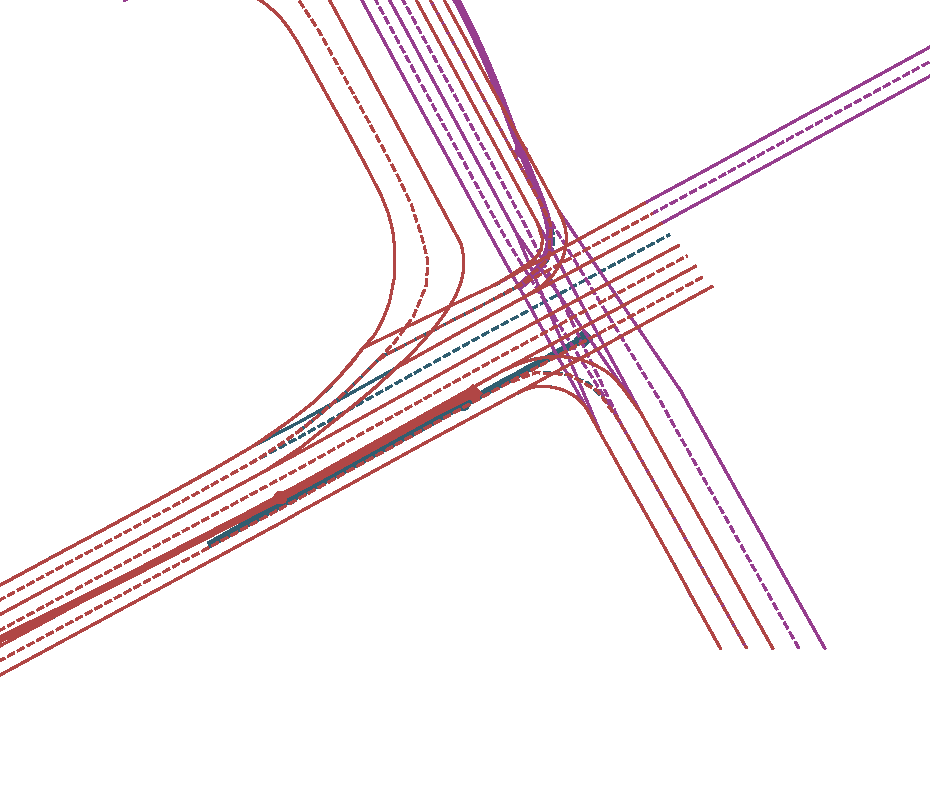
\includegraphics[width=0.32\linewidth]{chapter_7_Improving_Multi_Agent/qualitative/val_candidates_6_02b57064-6fe3-41a4-8ad5-24e51abbdac4.pdf} &
		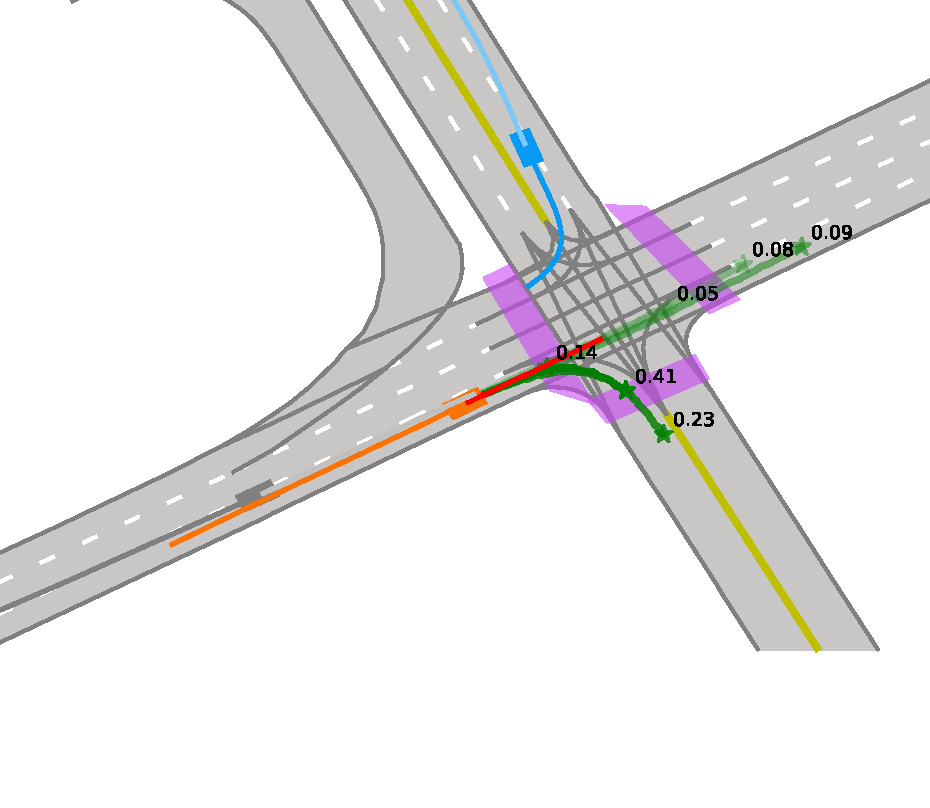
\includegraphics[width=0.32\linewidth]{chapter_7_Improving_Multi_Agent/qualitative/02b57064-6fe3-41a4-8ad5-24e51abbdac4_mm_prediction.pdf}
		\tabularnewline
		\tabularnewline
		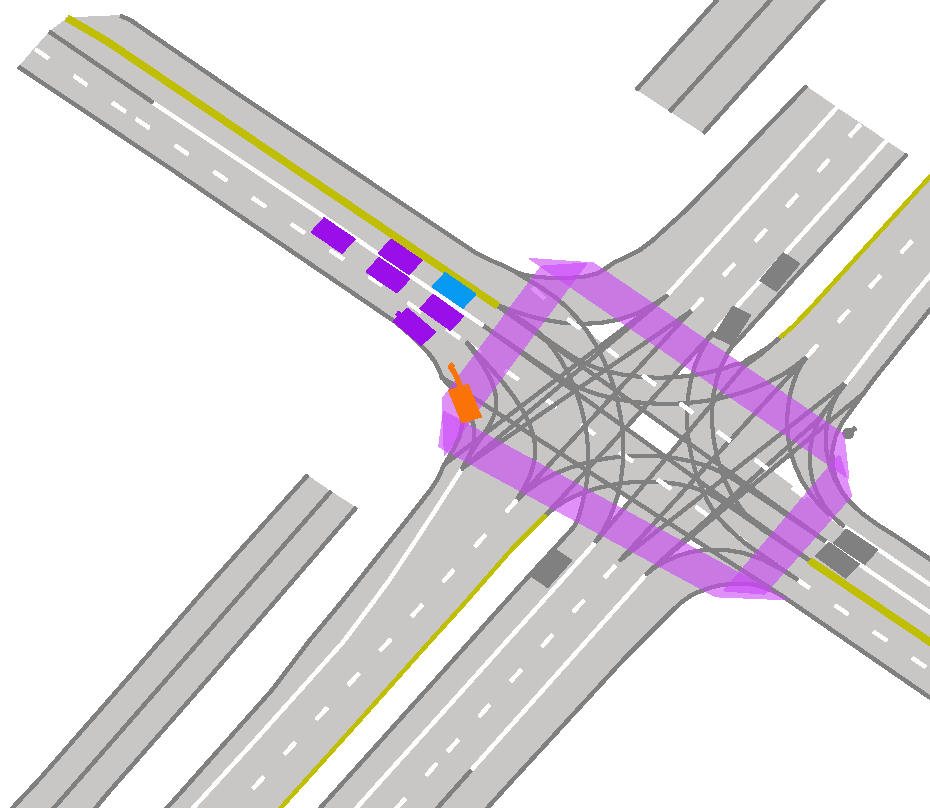
\includegraphics[width=0.32\linewidth]{chapter_7_Improving_Multi_Agent/qualitative/0499c82d-458b-464d-a603-e355e5da4ec7_input_data.pdf} & 
		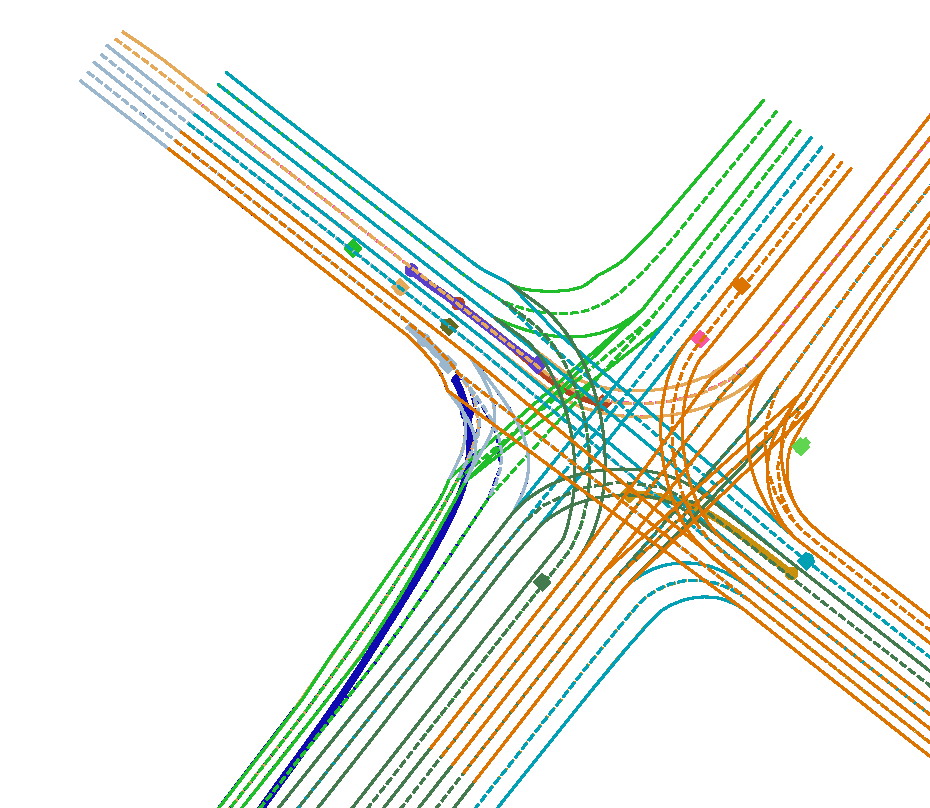
\includegraphics[width=0.32\linewidth]{chapter_7_Improving_Multi_Agent/qualitative/val_candidates_6_0499c82d-458b-464d-a603-e355e5da4ec7.pdf} &
		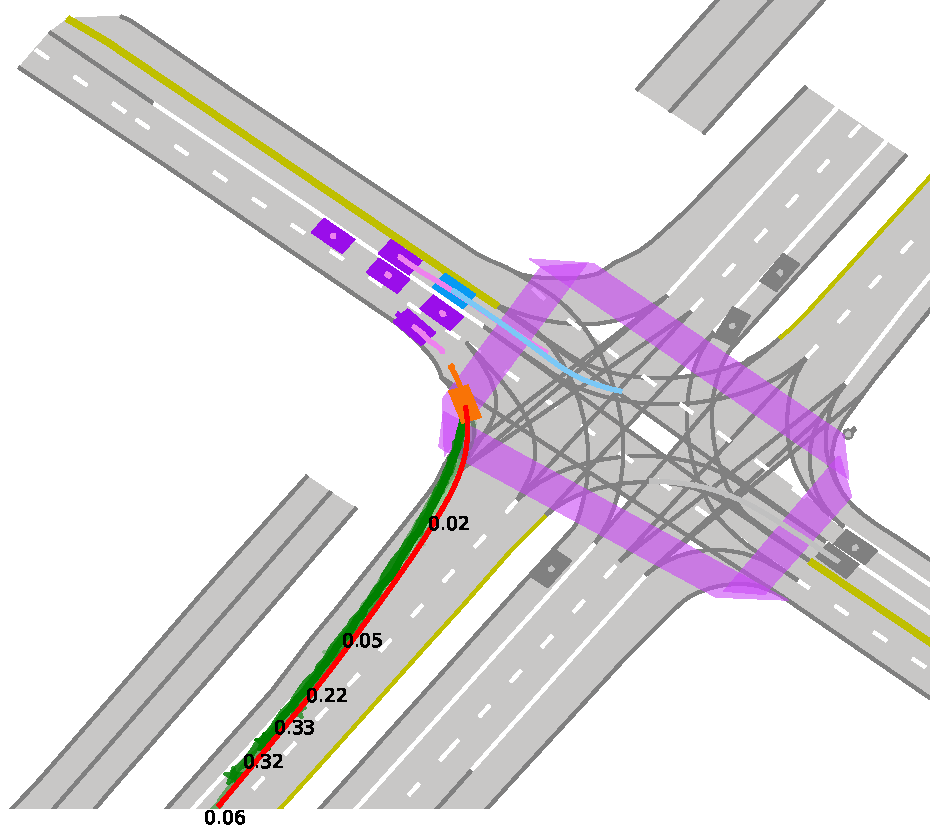
\includegraphics[width=0.32\linewidth]{chapter_7_Improving_Multi_Agent/qualitative/0499c82d-458b-464d-a603-e355e5da4ec7_mm_prediction.pdf}
		\tabularnewline
		\tabularnewline
		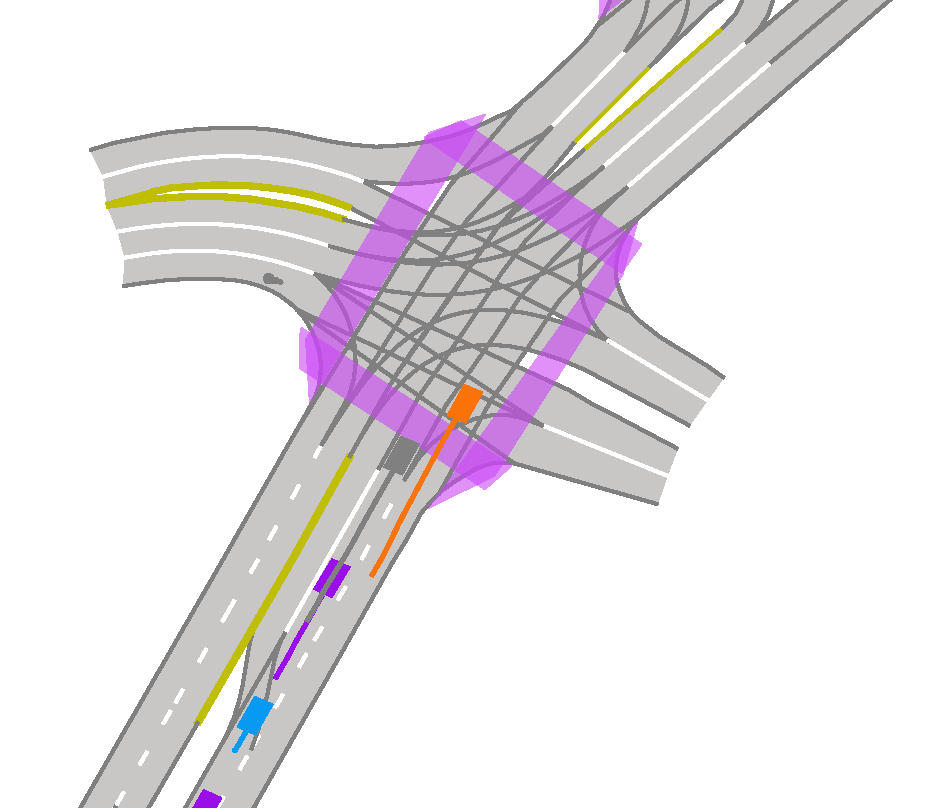
\includegraphics[width=0.32\linewidth]{chapter_7_Improving_Multi_Agent/qualitative/06f1ac5c-712f-4b37-ad17-6afaae41b753_input_data.pdf} & 
		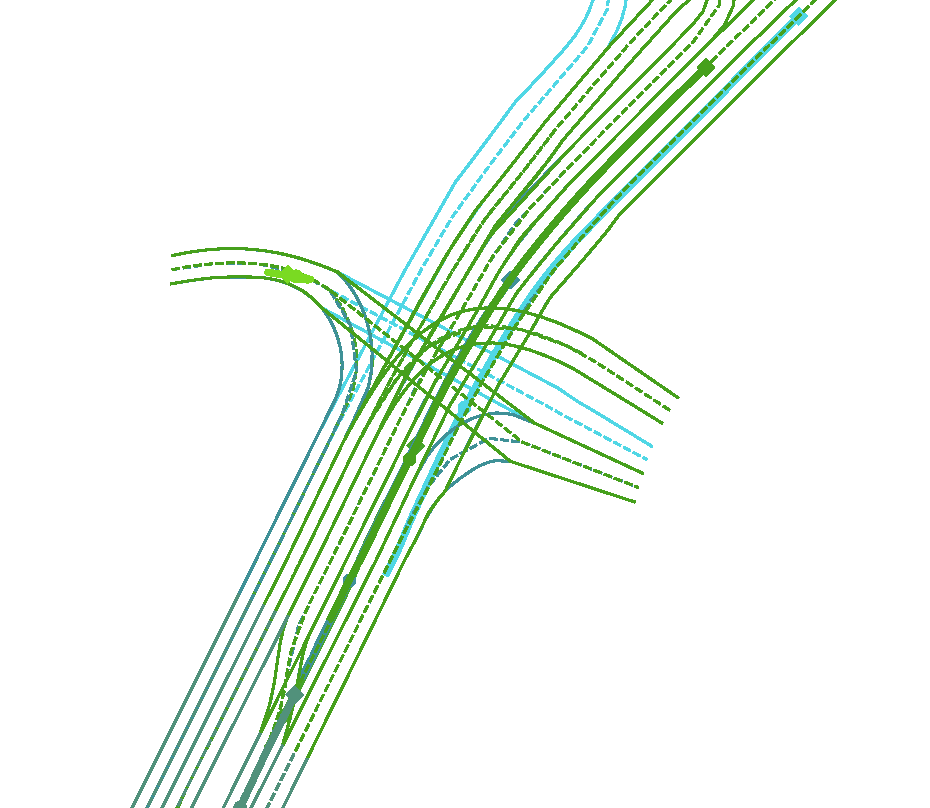
\includegraphics[width=0.32\linewidth]{chapter_7_Improving_Multi_Agent/qualitative/val_candidates_6_06f1ac5c-712f-4b37-ad17-6afaae41b753.pdf} &
		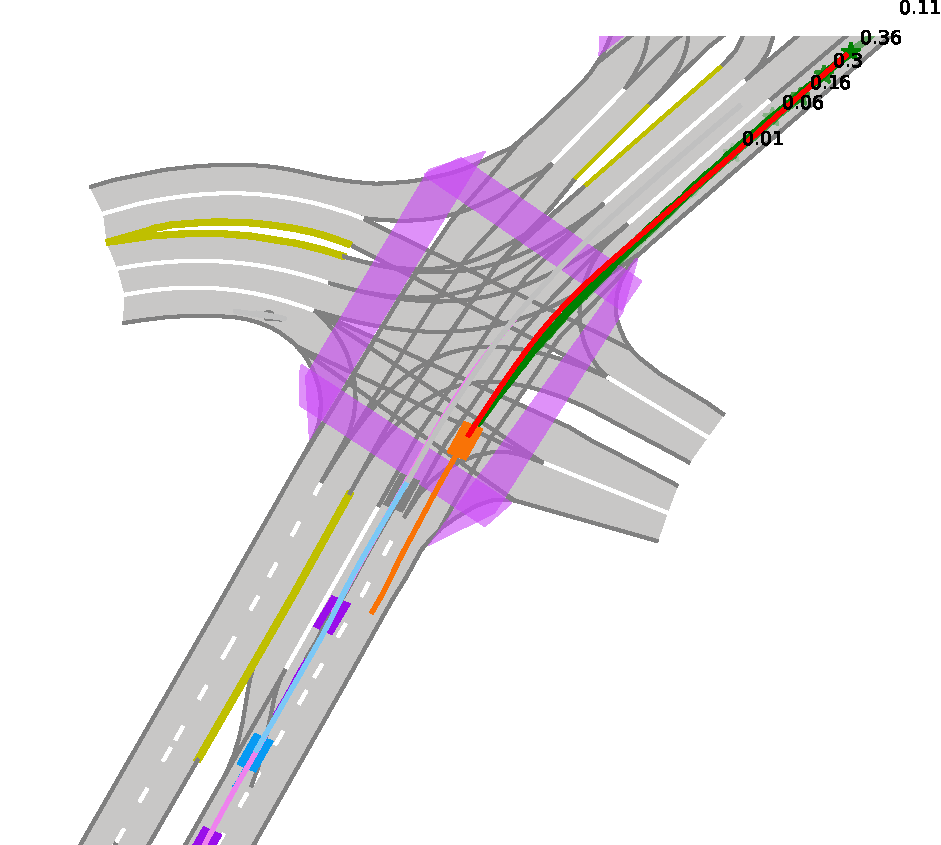
\includegraphics[width=0.32\linewidth]{chapter_7_Improving_Multi_Agent/qualitative/06f1ac5c-712f-4b37-ad17-6afaae41b753_mm_prediction.pdf}
		%
		\tabularnewline
		\tabularnewline
		HD Map input & Heuristic proposals & Multimodal (k=6) predictions \tabularnewline
	\end{tabular}
	\captionsetup{justification=justified}
	\caption[Qualitative Results on challenging scenarios in Argoverse 2 using our best model]{Qualitative Results on challenging scenarios in Argoverse 2 using our best model. We represent: our vehicle (\textbf{\textcolor{blue}{ego}}), the \textbf{\textcolor{YellowOrange}{focal agent}}, the \textbf{\color{blue-violet}{relevant agents}} in the scene, and \textbf{\textcolor{gray}{other agents}}. We can also see the \textbf{\textcolor{red}{ground-truth}} trajectory of the target agent, our \textbf{\textcolor{ForestGreen}{multimodal predictions}} (with the corresponding \textbf{confidences}). We also highlight the most important topology of the road, such as {\color{blue-violet}{pedestrian crossing}} and boundaries mark type. We show, from left to right, a general view of the traffic scenario (including and map information), the heuristic proposals for each agent (we only include the \textbf{\textcolor{blue}{ego}} and \textbf{\textcolor{YellowOrange}{focal agent}} for simplicity) and the multimodal prediction (\textit{k} = 6) for the \textbf{\textcolor{YellowOrange}{focal agent}}, including the corresponding confidences (the higher, the most probable)}
	\label{fig:chapter_7/argoverse_2_qualitative_results}
\end{figure}

\section{Summary}
\label{sec:7_summary}

In this Chapter we solve the challenging problem of Multi-Agent Motion Prediction in real driving scenarios. We present an end-to-end pipeline that combines Deep Learning (DL) and heuristic scene understanding. Our model uses as input the map of the scene, the past trajectories of the agents, and additional information about the scene geometry and agents e.g., type of agent, lane distribution. We propose a model that integrates attention mechanisms with GNNs, heuristic goals, and a motion refinement module to further improve temporal consistency. We achieve SOTA results on the Argoverse 2 Motion Forecasting Benchmark reducing in millions of parameters previous methods such as GANet, and improving over LaneGCN. Our code is publicly available. As future works, we plan to include map-adaptive lane-loss to improve diverse multiple motion prediction and explore knowledge-distillation to improve the efficiency for real-world deployment.